% Koma class
\documentclass[a4paper, oneside]{scrartcl}   

\usepackage{a4wide}

%------------------
% language = english
\usepackage[english, german]{babel}	% Umlaute mit \"u
\usepackage[latin1]{inputenc}
\usepackage{enumitem}

% margins + Kopf- und Fusszeilen
\usepackage[left = 2.5cm, right = 2.5cm, top = 2cm, bottom = 3cm]{geometry}
\usepackage{scrpage2} 
\pagestyle{scrheadings}
\clearscrheadfoot
\rehead{\headmark}
\lehead{\pagemark}
\lohead{\headmark}
\rohead{\pagemark} 

% math
\usepackage{amssymb}
\usepackage{amsmath}

% figures
\usepackage{tikz}
\usepackage{graphicx}

% section-Zaehler wird neu gesetzt:
\setcounter{section}{9}
%------------------
\author{Sascha Meiers, Martin Seeger}
\title{Exercise 9, Discrete Mathematics for Bioinformatics}
\date{Winter term 2011/2012}


\begin{document}
\maketitle

%---------------------------------------------------------------------------------------------------

\subsection{PORTA --- Polyhedron Representation Transformation Algorithm}

\renewcommand{\labelenumi}{\alph{enumi})}
\begin{enumerate}
    \item 
\begin{verbatim}
$ soplex -x problem.lp

Solution value is: 2.5000000e+00

Primal solution (name, id, value):
x2	1	1.5000000e+00    
x3	2	5.0000000e-01    
x4	3	5.0000000e-01    
All other variables are zero (within 1.0e-09).
\end{verbatim}

    \item Input file:
\begin{verbatim}
DIM = 4

LOWER_BOUNDS
0 0 0 0
UPPER_BOUNDS
2 2 1 1         \ We derived these bounds from the inequalities.

INEQUALITIES_SECTION
x1 + x2 + x3      <= 2
x1 + x2      + x4 <= 2
          x3 + x4 <= 1
END\end{verbatim}
Output file of \emph{vint}:
\begin{verbatim}
DIM =  4

CONV_SECTION
(  1) 0 0 0 0 
(  2) 0 0 0 1 
(  3) 0 0 1 0 
(  4) 0 1 0 0 
(  5) 0 1 0 1 
(  6) 0 1 1 0 
(  7) 0 2 0 0 
(  8) 1 0 0 0 
(  9) 1 0 0 1 
( 10) 1 0 1 0 
( 11) 1 1 0 0 
( 12) 2 0 0 0 

END\end{verbatim}
    These are all feasible points.


    \item \emph{traf} transforms these points into a inequality-representation:
\begin{verbatim}
DIM = 4

VALID
2 0 0 0 

INEQUALITIES_SECTION
(  1) -x1          <= 0
(  2)    -x2       <= 0
(  3)       -x3    <= 0
(  4)          -x4 <= 0
(  5)       +x3+x4 <= 1
(  6) +x1+x2+x3+x4 <= 2

END
\end{verbatim}


    \item We solve the new LP using \emph{soplex} and get:
\begin{verbatim}
Solution value is: 2.0000000e+00

Primal solution (name, id, value):
x1	0	2.0000000e+00    
All other variables are zero (within 1.0e-09).
\end{verbatim}
    

\end{enumerate}



\subsection{Branch and Bound}

\begin{enumerate}
  \item 
\begin{verbatim}
$ lp_solve -S3 example2.lp 

Value of objective function: 22.4

Actual values of the variables:
x1                            2.8
x2                              0
x3                              0
x4                              0

Actual values of the constraints:
c1                             14
\end{verbatim}
  \item 
  
We manually find a solution $(0,1,1,1)$, which is feasible, 
since $7 \cdot 1 + 4 \cdot 1 + 3 \cdot 1 \leq 14$, 
and gives a \textbf{global lower bound} for the ILP of $21$.

The solution of the LP-relaxation (with all variables bound to $0 \leq x_i \leq 1$)
gives an optimal value of $22$ in the point $(1,1,0.5,0)$. 
Since the variables are not integral we start branching now:

\begin{center}
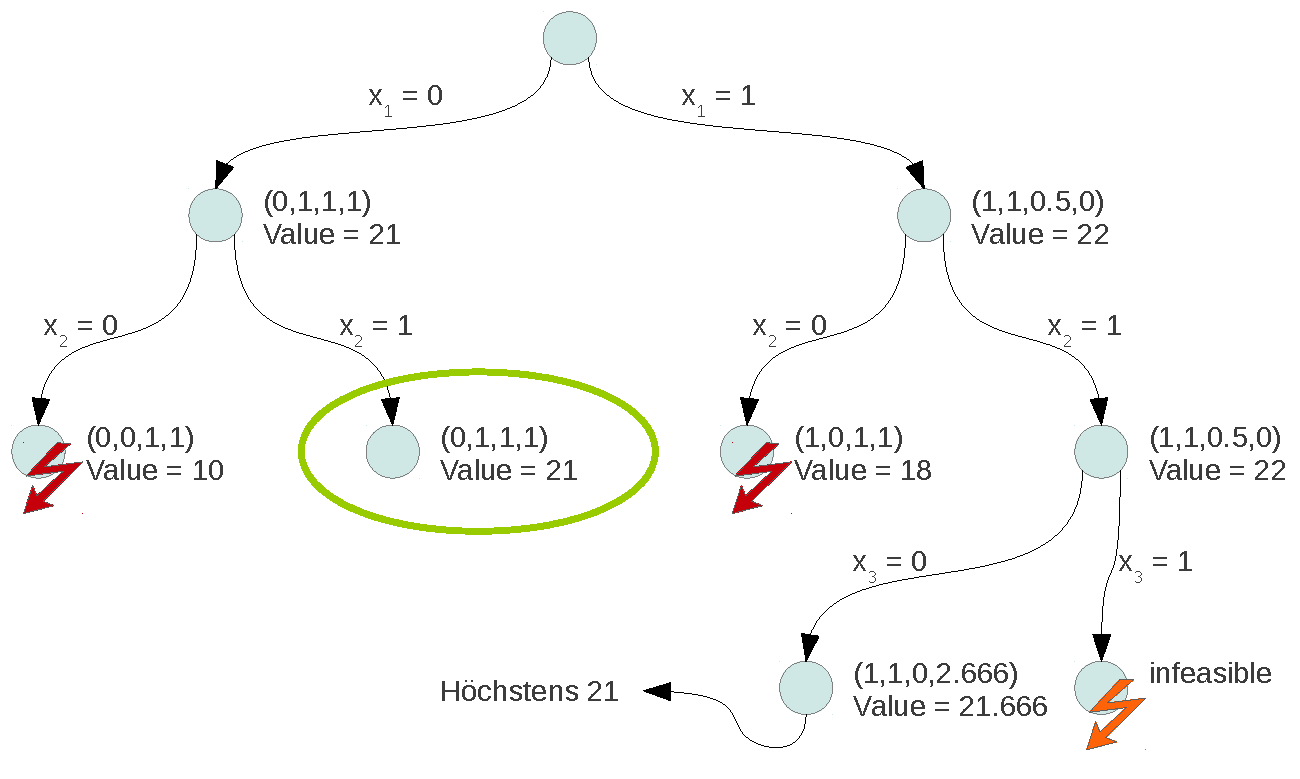
\includegraphics[width=\textwidth]{branchANDbound_ex9.pdf}
\end{center}


\end{enumerate}

\end{document}
